
\section{Experimental Setup}

    %Explain your program purpose
    I specifically wanted to capture different program patterns that captures the following features
    \begin{itemize}
        \item Captures Read-Write, Read-Read, Write-Read, Write-Write dependencies between shared memory.
        \item Logical resources (adders) used by such programs.
        \item Mixture of shared and local memory usage.
    \end{itemize}

    Since I assume my programs have no conditionals or loops, I wanted to capture relatively general program patterns that may possibly occur while performing optimizations. 
    To capture all the above features, the following program format deemed sufficient as that in Fig~\ref{P1}.
    \begin{figure}[H]
        \centering
        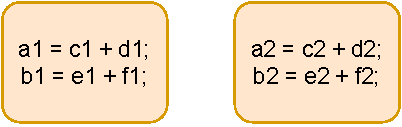
\includegraphics[scale=0.5]{Prog.pdf}
        \caption{Program Format}
        \label{P1}
    \end{figure}

    For each of the above accesses, I create a program where either they are shared or not. 
    For example, $a1$ can be either just $a1$ or $as$ (in this way, I capture the notion of shared memory between the two threads, since $a2$ may also become $as$.)
    This way, in total, I get 4096 programs. 

    %How it represents the patterns the compiler optimization would have 

    %Show how it covers the MP, SB, LB ordering patterns 

    %Show how it covers the resource constraint problem 

    %Detail the stats (how maby programs, how many sharred accesses, etc)